%
% teilNeu2.tex -- Beispiel-File für Teil 2
%
% (c) 2020 Prof Dr Andreas Müller, Hochschule Rapperswil
%
% !TEX root = ../../buch.tex
% !TEX encoding = UTF-8
%
\section{Mathematische Grundlagen
\label{helmholtz:section:Mahtematische_Grundlagen}}
\kopfrechts{Mathematische Grundlagen}

Hier werden kurz die Tools vorgestellt, welche für die Helmholtz-Zerlegung
benötigt werden.
Um die Helmholtz-Zerlegung in der Akustik zu verstehen, ist ein
solides Verständnis der grundlegenden mathematischen Konzepte
notwendig.
In diesem Abschnitt werden die wichtigsten Vektoroperatoren und
ihre Eigenschaften vorgestellt, die für die Zerlegung von Vektorfeldern
benötigt werden.

\subsection{Vektorfelder und Operatoren
\label{helmholtz:subsection:Vektorfelder_Operatoren}}

Vektorfelder stellen in jedem Punkt eines Raumes einen Vektor dar,
der sowohl eine Richtung als auch einen Betrag besitzt.
In der Akustik sind Vektorfelder von zentraler Bedeutung, da sie
physikalische Größen wie die Schallschnelle und die Intensität
beschreiben.
Um diese Felder zu analysieren, werden spezielle Operatoren verwendet,
die lokale Eigenschaften des Feldes charakterisieren.

\subsubsection{Der Gradient eines Skalarfeldes}

Der Gradient eines Skalarfeldes $a$ ist ein Vektorfeld, das in jedem
Punkt in Richtung des steilsten Anstiegs von $a$ zeigt.
Mathematisch wird der Gradient durch die Gleichung
\begin{equation}
\nabla a (\boldsymbol{r})
=
\frac{\partial a}{\partial x}\boldsymbol{e}_x
+
\frac{\partial a}{\partial y}\boldsymbol{e}_y
+
\frac{\partial a}{\partial z}\boldsymbol{e}_z
\end{equation}
definiert.



\subsubsection{Die Divergenz eines Vektorfeldes}

Die Divergenz eines Vektorfeldes $\boldsymbol{F}$ ist ein Skalarfeld,
das beschreibt, wie stark Feldlinien auseinanderstreben oder
zusammenlaufen.
Sie wird durch die Formel
\begin{equation}
\nabla \cdot \boldsymbol{F}(\boldsymbol{r})
=
\frac{\partial F_x}{\partial x}
+
\frac{\partial F_y}{\partial y}
+
\frac{\partial F_z}{\partial z}
\end{equation}
ausgedrückt.
Die Divergenz kann als Mass für die Quellen- oder Senkenstärke an
einem bestimmten Punkt im Vektorfeld interpretiert werden.
Ein Bereich mit positiver Divergenz stellt eine Quelle dar, aus der
Feldlinien hervorgehen, während ein Bereich mit negativer Divergenz
eine Senke darstellt, in der Feldlinien zusammenlaufen, wie in
Abbildung \ref{fig:DivergenzAlg} dargestellt.

\begin{figure}
    \centering
    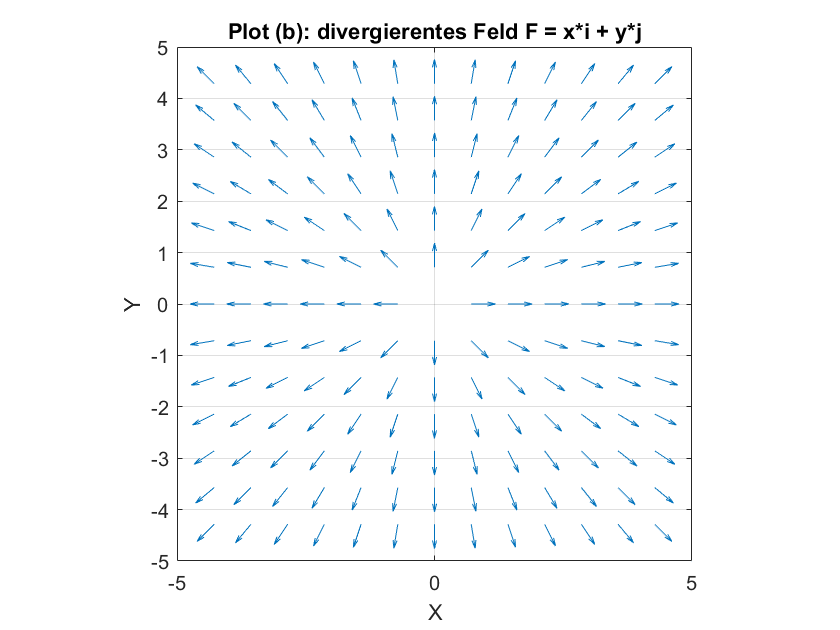
\includegraphics[scale=0.4]{papers/helmholtz/images/divergentes_Feld.png}
    \caption{Beispiel eines divergenten Vektorfeldes, das Quellen und Senken aufweist}
    \label{fig:DivergenzAlg}
\end{figure}

\subsubsection{Die Rotation eines Vektorfeldes}

Die Rotation eines Vektorfeldes $\boldsymbol{A}$ ist ein Vektorfeld,
das die Wirbeldichte des ursprünglichen Feldes beschreibt.
Sie wird definiert als
\begin{equation}
\nabla \times \boldsymbol{A}(\boldsymbol{r}) = \begin{vmatrix}
    \boldsymbol{e}_x & \boldsymbol{e}_y & \boldsymbol{e}_z \\
    \frac{\partial}{\partial x} & \frac{\partial}{\partial y} & \frac{\partial}{\partial z}\\
    A_x & A_y & A_z
\end{vmatrix}.
\end{equation}
Die Rotation misst, wie stark sich die Feldlinien um eine Achse
drehen und gibt sowohl die Achsenorientierung als auch die Stärke
eines solchen Wirbels an, wie in Abbildung \ref{fig:RotationAlg}
zu sehen ist.

\begin{figure}
    \centering
    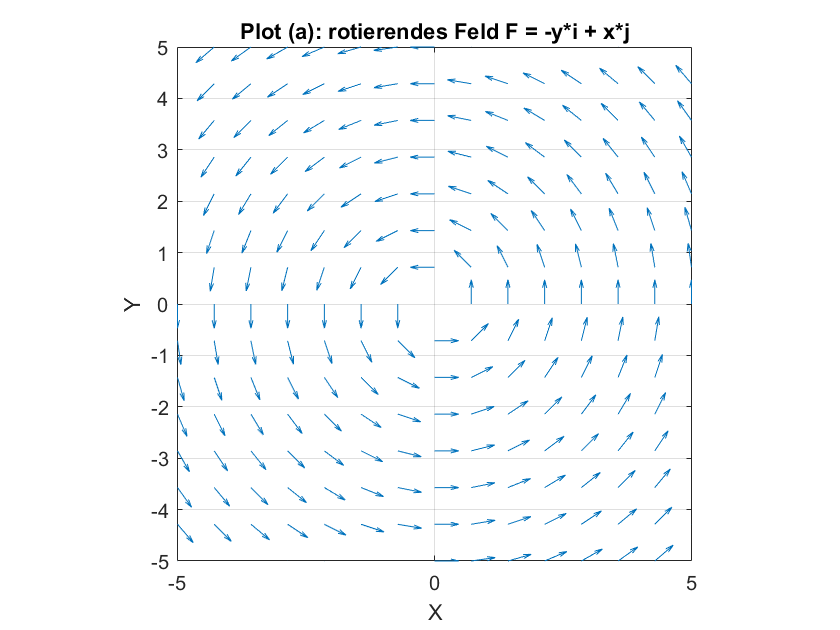
\includegraphics[scale=0.4]{papers/helmholtz/images/rotierendes_Feld.png}
    \caption{Beispiel eines rotierenden Vektorfeldes mit deutlich erkennbarer Wirbelstruktur}
    \label{fig:RotationAlg}
\end{figure}

\subsubsection{Der Laplace-Operator}

Der Laplace-Operator, oft als $\nabla^2$ oder $\Delta$ geschrieben,
ist ein skalarer Differentialoperator zweiter Ordnung.
Angewendet auf ein Skalarfeld $a$ ergibt er
\begin{equation}
\nabla^2 a(\boldsymbol{r}) = \frac{\partial^2 a}{\partial x^2} + \frac{\partial^2 a}{\partial y^2} + \frac{\partial^2 a}{\partial z^2}.
\end{equation}
Der Laplace-Operator spielt eine zentrale Rolle in vielen physikalischen Gleichungen, insbesondere in der Potentialtheorie und der Wellenausbreitung.
Für ein Vektorfeld $\boldsymbol{F}$ wird der Laplace-Operator
komponentenweise angewendet und das Resultat kann wie in
Abbildung~\ref{fig:LaplaceAlg} dargestellt aussehen.
Die Formel für den Laplace-Operator ist
\begin{equation}
\nabla^2 \boldsymbol{F} = (\nabla^2 F_x)\boldsymbol{e}_x + (\nabla^2 F_y)\boldsymbol{e}_y + (\nabla^2 F_z)\boldsymbol{e}_z.
\end{equation}

\begin{figure}
    \centering
    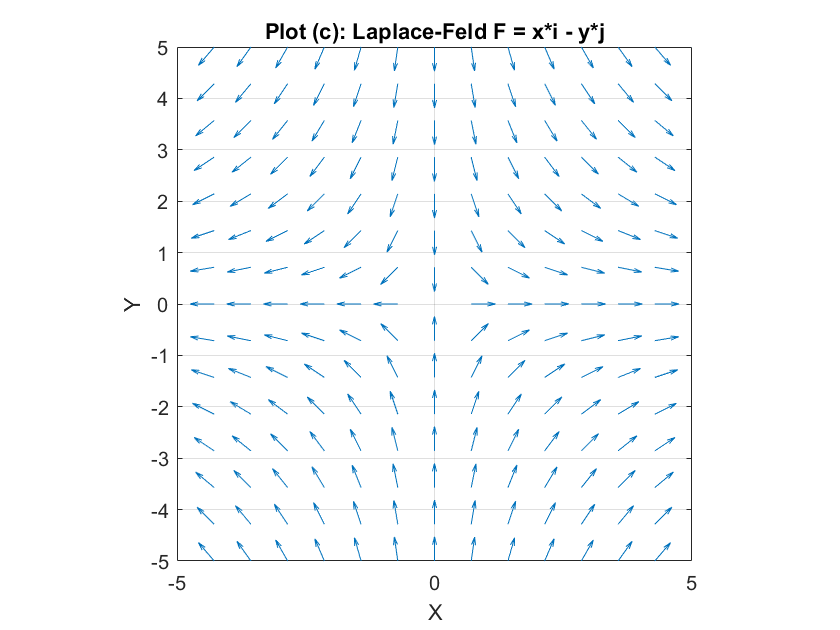
\includegraphics[scale=0.4]{papers/helmholtz/images/Laplace_Feld.png}
    \caption{Visualisierung des Laplace-Operators auf ein Skalarfeld}
    \label{fig:LaplaceAlg}
\end{figure}


\subsection{Vektoridentitäten
\label{helmholtz:subsection:Vektoridentitaeten}}
Für die mathematische Herleitung der Helmholtz-Zerlegung werden
verschiedene Vektoridentitäten benötigt.

\subsubsection{Wichtige Vektoridentitäten}

Die folgenden Identitäten sind für die Ableitung der Helmholtz-Zerlegung besonders relevant:

\begin{itemize}
\item Für jedes Skalarfeld $\Phi$ gilt: $\nabla \times (\nabla \Phi) = 0$.
\item Für jedes Vektorfeld $\boldsymbol{F}$ gilt: $\nabla \cdot (\nabla \times \boldsymbol{F}) = 0$.
\item Der Laplace-Operator eines Vektorfeldes lässt sich umformen zu:
\begin{equation}
\nabla^2 \boldsymbol{F} = \nabla(\nabla \cdot \boldsymbol{F}) - \nabla \times (\nabla \times \boldsymbol{F}).
\end{equation}
Diese Identität ist fundamental für die Ableitung der Helmholtz-Zerlegung.
Sie wurde als \eqref{buch:vektoranalysis:eqn:rotrot} in
Abschnitt~\ref{buch:vektoranalysis:subsetion:operatorrelationen} hergeleitet.
\end{itemize}




